\section{Exp4: Pushing task in simulation II}

To not enforce any constraints on the shape of the Q-function, experiments were
done with Deep Deterministic Policy Gradient (DDPG) where the Q-function can be
approximated by any differentiable function without any theoretical constraints
(see section \ref{sec:ddpg}). Also, simplifications regarding translations, and
rotations, of the problem were taken advantage of.

\subsection{Environment}

The environment is in the basic aspects the same as for the experiments in
section \ref{sec:push_sim_1}. The reward was however changed and consisted of
three parts:

\begin{equation}
    r(s, u, s') = k_1 \left(\mathbf{||c - g|| - ||c' - g||}\right) + k_2 \exp \lbrace -k_3 ||c' - g|| \rbrace + k_4 \exp \lbrace -k_5||e' - c'||\rbrace
\end{equation}

The vectors $\mathbf{e, c}$ and $\mathbf{g}$ are inferred from the state $s$
and are the poses of the end-effector, pushable object, and the goal. The prime
notation represents the successor state. To simplify the task for the learning
agent, the state representation and action space was changed to become rotation
and translation invariant. The environment was translated so that the pushable
object was positioned at the origin, and rotated so that the goal position lies
on the negative x-axis, see figure \ref{fig:ddpg-coordinates}. Actions in the
environment were interpreted in this new coordinate frame.

\begin{figure}[h!]
    \centering
    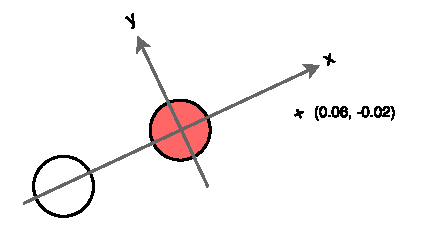
\includegraphics[width=0.5 \textwidth]{res/ddpg-coordinates.pdf}

    \caption{The environment is translated and rotated so that the agent sees the same
    problem, invariant of translations and rotations. The state of the environment
    reduces to three dimensions, the distance from the pushable object (red) to the
    goal position (white), and the coordinates of the end-effector/pointer (+) in
    the new coordinate frame.}

    \label{fig:ddpg-coordinates}

\end{figure}


\subsection{Algorithms}

DDPG was used, where two separate networks represent an actor and critic
respectively. Both networks had two hidden layers with 400 units in the first
layer, and 300 in the second layer. Batch normalization was used on the input,
and between the two hidden layers. Activation functions were exponential linear
units (ELU) except for the Q-value and policy outputs which had linear and tanh
activation functions. The critic network was regularized using the L2-norm
multiplied by $10^{-2}$. Gradient descent was done on both networks using Adam
with learning rate $10^{-3}$ for the critic and $10^{-4}$ for the actor and the
other parameters set to the same as suggested by Kingma et al
\cite{kingma2014adam}. Parameters of target networks $(\theta')$ were updated
using soft updates $\tau = 10^{-3}$:

\begin{equation}
    \theta' \leftarrow \tau \theta + (1 - \tau) \theta'
\end{equation}

A priority buffer was used in the same manner as stated in section
\ref{sec:push_sim_1}. A single state transition was sampled from the
environment using the current policy with noise, followed by a single gradient
update for each of the networks from a sampled mini-batch and thereafter
applying soft update to the target networks. Actions were sampled with added
noise, using an $\epsilon$ linearly annealed from $1$ to $0.1$, according to:

\begin{equation}
    \mathbf{u} = (1 - \epsilon) \mathbf{\mu}(s) + \epsilon \left[U(-1, 1), U(-1, 1)\right]
\end{equation}

Action outputs from the networks were in the range $[-1, 1]$ and were scaled by
$0.01$ before being applied in the environment. Policies were evaluated by
estimating the return from sampled start states by regularly executing a set of
trials in the environment.

NAF was evaluated alongside DDPG with a separate replay buffer and environment
but with the same procedure otherwise. Several runs with NAF were done with
different sizes of hidden layers, using batch normalization, and changing to
ELU activations. The NAF experiments did however not succeed to show any signs
of converging at a good policy, and further results with NAF are omitted here.

\subsection{Results}

Good policies were found after approximately $30'000$ iterations, shown in
figure \ref{fig:ddpg-sim-pushing-pi-v} and \ref{fig:ddpg-sim-pushing-series}.
However, as can be seen in figure \ref{fig:ddpg-sim-pushing-returns}, estimated
returns varied greatly between runs despite weight initialization from the same
distributions. Also, it was common for good policies to be found, be
subsequent policies showed deteriorating estimated returns which did not
recover.

\begin{figure}[h!]
    \centering
    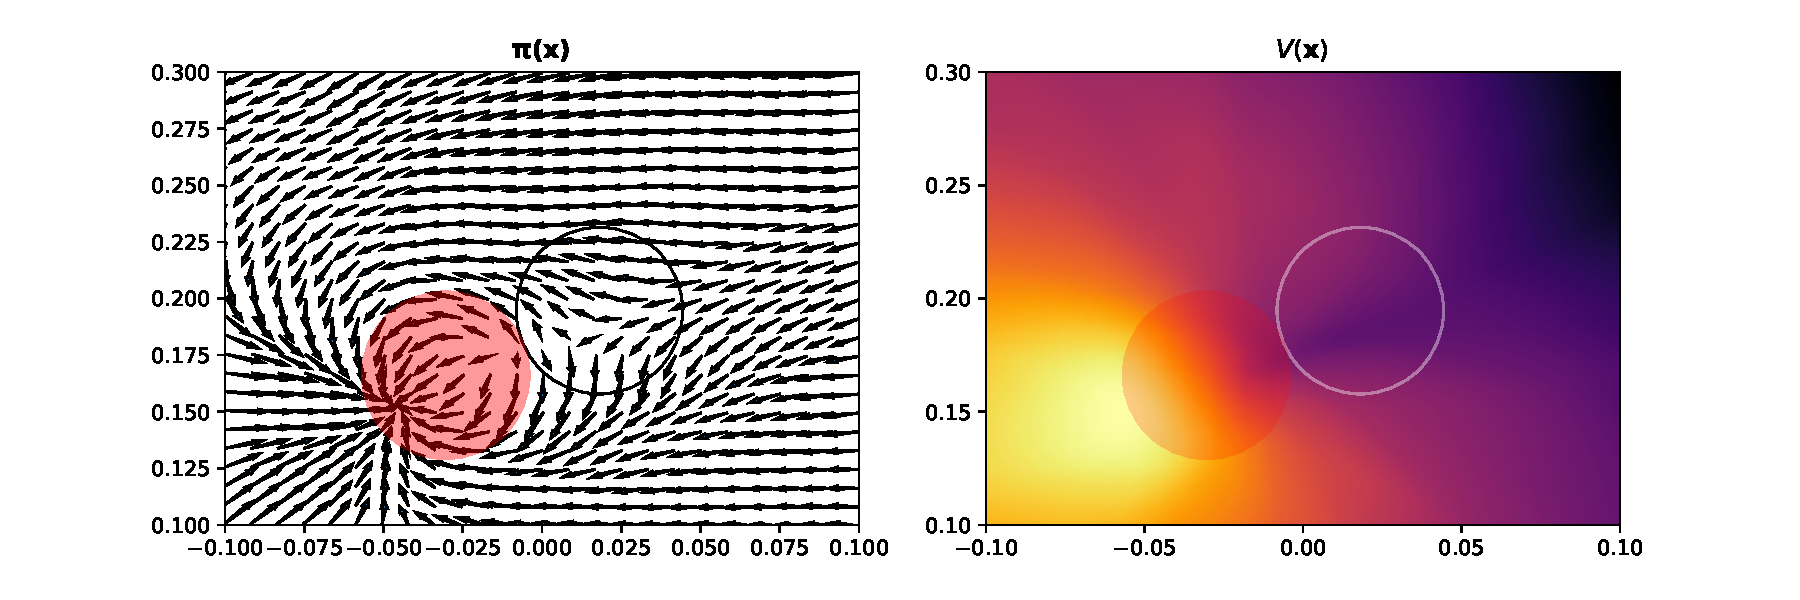
\includegraphics[width=1.0 \textwidth]{res/ddpg-pushing-pi-v.pdf}

    \caption{Trained policy and value function on a simulated pushing task
    using DDPG. The red circle is the pushable object, and the hollow circle is
    the goal. The value function was derived using $Q(\mathbf{x, \pi(x)})$}

    \label{fig:ddpg-sim-pushing-pi-v}

\end{figure}

\begin{figure}[h!]
    \centering
    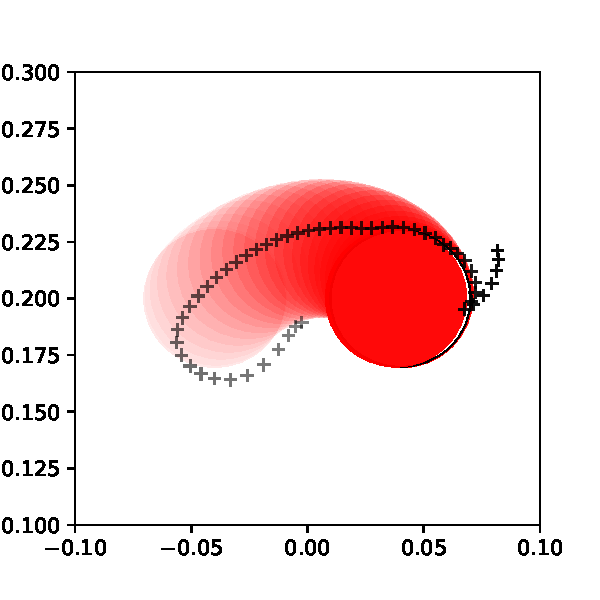
\includegraphics[width=0.49 \textwidth]{res/ddpg-sim-pushing-series1.pdf}
    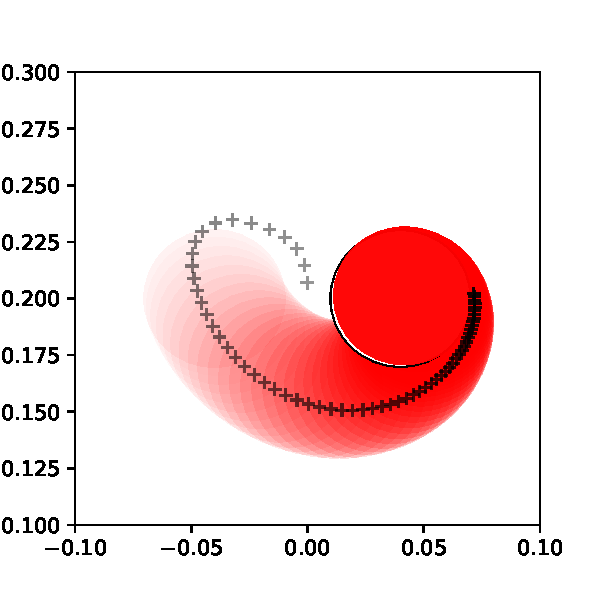
\includegraphics[width=0.49 \textwidth]{res/ddpg-sim-pushing-series2.pdf}

    \caption{The policy trained using DDPG manages to go around the object to
    push it towards the goal position.}

    \label{fig:ddpg-sim-pushing-series}

\end{figure}

\begin{figure}[h!]
    \centering
    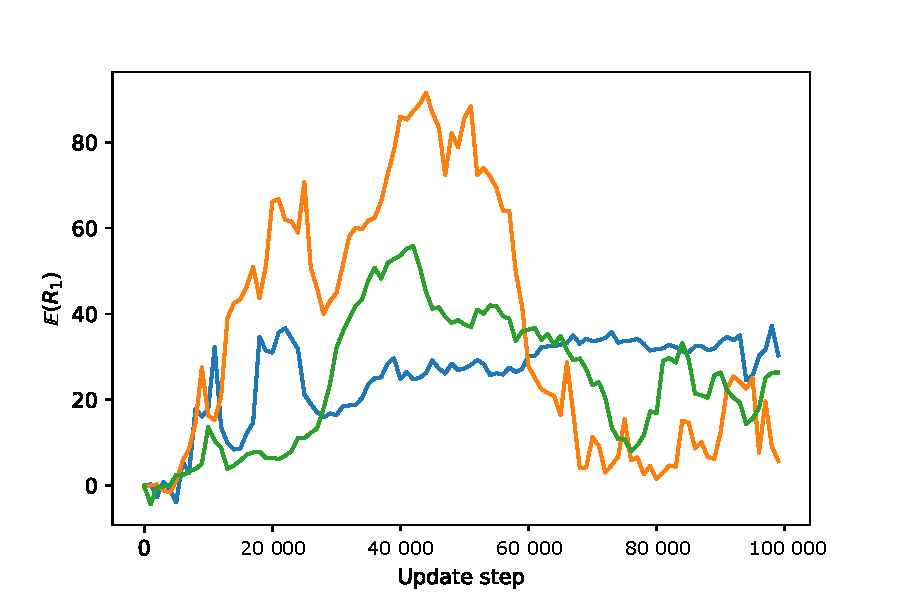
\includegraphics[width=0.6 \textwidth]{res/ddpg-pushing-sim-several-runs.pdf}

    \caption{The estimated returns of policies trained using DDPG showed large
    variations between runs even though network initializations were sampled
    from the same distributions. Also, a good policy could be found but then
    showed a ''crashing'' behavior for which the estimated returns did not seem
    to recover from.}

    \label{fig:ddpg-sim-pushing-returns}

\end{figure}
